\section{Abstract}
	The performance results for five different Garbage Collection (GC) algorithms for Non-Volatile Memory Devices for three access patterns are presented in this report. The access patterns include a long-tailed distribution as well as Uniform distribution. The results indicate that Round-Robin style GC algorithms perform much better in all cases than Generational algorithms. This is counter-intuitive to the existing norms. Invocation of the GC in Flash devices is determined by the fullness of the device. Even at low fullness levels, Generational GCs have very low efficiency. In this paper, we compare the efficiency and the time taken for the individual GCs at fullness levels ranging from 2\% to 98\%.  Existing research looks into using Flash as storage for data and RAM as cache \cite{Gupta09, Budilovsky11, Tjioe12}. We analyze the performance of a Flash when it is used in place of a RAM.

\subsection*{Keywords}
	Garbage Collection, Flash memory, Statistical access pattern.

%-----------------------------------------------------------------------------------
\section{Introduction}
	Flash memory is a powerful and cost-effective solid-state non volatile storage technology that is widely being used in mobile devices and other embedded devices. Compared to traditional Hard Disk Drives, they have low power consumption and a small size. Embedded devices are constrained by power and low memory capacity. Hence there is a need to have a very efficient primary storage system that allows fast read and write operations and thereby less power consumption. Flash devices generally have fast read accesses but have very slow write accesses. \\

\begin{center}
   \begin{tabular} {|  c | c | c | }
       \hline
	{\bf Read time(ms)} & {\bf Write time (ms)} & {\bf Erase time (ms)} \\ \hline
	4 & 5 & 6 \\ 
       \hline
   \end{tabular}
\end{center}

There are 2 major Flash devices available today - NAND and NOR. NAND flash has a very small cell size and is mainly used for storage of large amounts of data as its cost-per-bit is very low compared to NOR \cite{Toshiba}. NAND flash is organized into blocks and each block is divided into pages. Block size of a typical NAND flash is 16KB and the page size can be 512B (32 pages in a block). Read and Write operations happen take place on pages whereas erase happens on blocks. NOR flash on the other hand, have individual cells connected in parallel which allow it to achieve random access. This enables it to achieve short read times and allow individual bits to be set (called reprogramming). This has the advantage that it can execute code, a feature called eXecute-In-Place (XIP). \\

Every block on a NAND flash can be written-to or erased only a limited number of times (in order of 1 million or $10^6$ cycles). Writing to or erasing a block beyond this limit can result in "wearing" out of the Flash, which can lead to write failures or can return invalid data for read operations. Data cannot be written over already written areas (called in-place update). Data can only be written to areas that have already been erased. Therefore if some data has to be updated on the flash, it is first written to a new area and the old data is marked invalid. This is called out-of-place-update. After many cycles of writes, the entire flash is fragmented with valid and invalid data and the flash quickly runs out of space for new data. This is when the Flash invokes the Garbage Collector whose task is to collect all valid data in a block, write it to a new location and erase the old block. This paves the way for new data to be written to the flash. But this operation of moving data to a new location and erasing a block is costly and has to be kept to a minimum. Based on the above points, some of the challenges for a good GC algorithm is: (a) To maintain "wear-levelling" of the flash blocks (b) Reduce the amount of time taken to move data and erase blocks.

\begin{center}
\captionof{table}{A comparison of NAND and NOR Flash} \label{NANDvsNOR}
   \begin{tabular} {|  c | c | c | }
       \hline
	{\bf Design Characteristic} & {\bf NAND flash} & {\bf NOR Flash} \\ \hline
	Cost-per-bit & Low & High \\ \hline
	File Storage use & Easy & Hard \\ \hline
	Code execution & Hard & Easy\\ \hline
	Capacity & High & Low\\ \hline
	Write speed & High & Low\\ \hline
	Read speed & Medium & High\\ \hline
	Active power & Low & High\\ \hline
	Standby power & Medium & Low\\
       \hline
   \end{tabular}
\end{center}

Table~\ref{NANDvsNOR} compares the characteristics of NAND and NOR Flash devices \cite{Toshiba}. 
\\

An important component that has an overhead and affects the performance of the storage system is the Garbage Collector (GC) algorithm. This report quantifies the performance of different GCs against different statistical traffic patterns such as Uniform, Pareto and Bi-Modal. Based on prior experiments, we have observed that the traffic pattern for the data can occur in short bursts or can arrive at regular intervals. This is the reason why we chose to select the afore-mentioned traffic patterns. A simulator for the Flash file system as well as the GC algorithms were coded in Matlab. We compare the performance of five different GC algorithms against three traffic patterns. Our experiments indicate that Round-Robin style algorithms have better efficiency than Generational algorithms.\\

There are three major GC algorithms that have been studied for Log-Structured File Systems - Greedy, Cost-Benefit analysis and Cost-Age Time (CAT). Greedy algorithms select those data blocks that can yield the most free space, whereas a cost-benefit algorithm selects blocks based on the free space as well as the age of the segment \cite{Menon98, Kwon07}. CAT reduces the erase operations by segregating the hot from the cold data \cite{Chiang99}. A major advantage of this approach is that it takes wear-levelling into account before cleaning a block. \\

In Solid State Devices such as NAND and NOR based Flash, new data is always written out-of-place. In a Log-Structured File System, this reduces the amount of free space and a Garbage Collector algorithm is invoked which defragments the device by moving all valid data together and erasing the invalid data. This is a critical factor in the performance and life-time of a Flash device. In this paper, we present our work in analyzing five different GC algorithms and compare their performances against various parameters. We also present the theoretical model behind our simulation and explain the reason behind the results we have obtained. A major contribution of our work is to measure the performance of Flash devices against traffic patterns that are generally observed in practice. \\
The major goals of our work are:
\begin{itemize}
\item To find out if Flash can work as a good primary storage system. 
\item To create performance benchmarks and understand which Garbage Collection algorithm is better. 
\item To create statistical models to test the GC algorithms.
\end{itemize}

We simulated an application which is both equally read and write dominant. We also tested an application which has only writes.

The report is organized as follows: section 3 gives details on related work being conducted currently. Section 4 mentions about the current state-of-the-art in Flash algorithms and section 5 provides details on the Mathematical models behind our simulations. We conclude by outlining our results in section 6, details about our simulator in section 7 and finally talk about future work in this area.

%-----------------------------------------------------------------------------------
\subsection{Log Structured File System}
	Due to increasing capacity and reduction in accessing times of RAM, reads have become quite fast and writes take up bulk of the time in a typical embedded device. Hence there is a need for a file system that provides fast write access. A \emph{log structured file system} is one such system that writes data sequentially in a log-like manner \cite{Rosenblum91}. This reduces the write time as there is no structure other than logs in a device to be maintained and thereby reducing the amount of data seeks. But in order for a log-structured file system to operate efficiently, it needs to have large amounts of free space to write new data. LFS also allow fast recovery from crashes which is not present in traditional file systems as they have to scan the entire set of data in order to build the index.

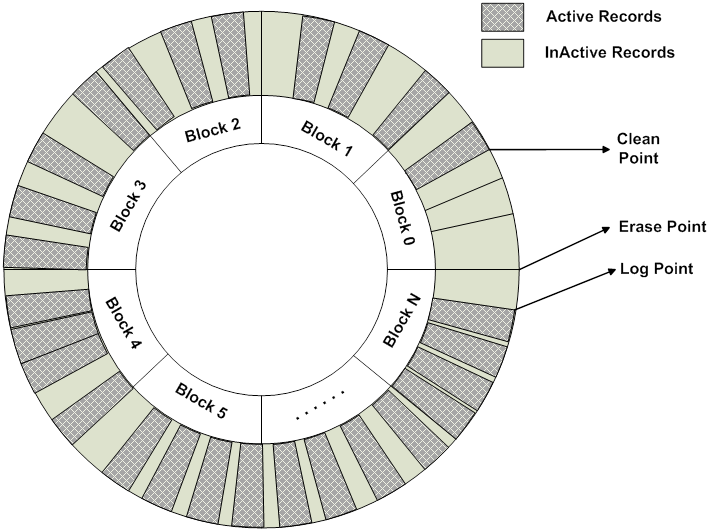
\includegraphics [width=3.5in,height=2.5in] {C:/Ananth/OSU/CETI/MS-Thesis/MS-thesis-Report/imgs/Flash-Block-structure.png}

%-----------------------------------------------------------------------------------
\subsection{Methodology}
The GC and the applications will be implemented in Matlab 2011b. The tests will be run on the Ohio Super Computer center’s cluster called Oakley. The fullness level will range from 2% to 98% and the simulations will run for 100,000 read/write accesses per fullness level. The simulations are done for all three traffic patterns for all 6 GC algorithms.

%-----------------------------------------------------------------------------------
\subsection{Implementation details:}
The application generates random records and sizes using the rand() function in Matlab. For Pareto distribution, each record is assigned a weight which decides the usage of a record. After the records are generated, based on a coin toss, it is decided whether the next operation will be a read or a write. Every time the GC is accessed, details such as amount of bytes moved, blocks erased, are captured. These details are then used to plot the required graphs. 

%-----------------------------------------------------------------------------------
\section{Related Work}


